\chapter{\sffamily Interacting with systems in general}

{\bfseries\sffamily Concept.} To design and build a software which can interact with stochastic processes of any kind, either manually through user input, or automatically by introducing a `policy'. The mathematical formalism and software that we introduce here will serve as a common language and interface for any simulation studies into manipulating real world phenomena, and will enable the learning of control algorithms in later chapters of this book. We will implement this new interaction software as an extension to the stochadex package. For the mathematically-inclined, this chapter will cover how interactions are structured in theory by adding some new concepts to the stochadex formalism and illustrating with some simple examples. For the programmers, the public Git repository for the code described in this chapter can be found here: \href{https://github.com/umbralcalc/stochadex}{https://github.com/umbralcalc/stochadex}.

\section{\sffamily Formalising general interactions}

Let's start by considering how we might adapt the mathematical formalism we have been using so far to be able to take actions which can manipulate the state at each timestep. Using the mathematical notation that we inherited from the stochadex, we may extend the formula for updating the state history matrix $X_{0:{\sf t}}\rightarrow X_{0:{\sf t}+1}$ to include a new layer of possible interactions which is facilitated by a new vector-valued `take action' function $G_{{\sf t}}$. In doing so we shall be defining the domain of an acting entity in the stochastic process environment --- which we shall hereafter refer to as simply the `agent'.

During a timestep over which actions are performed by the agent, the stochadex state update formula can be extended to include interactions by composition with the original state update function like so
%%
\begin{align}
X_{{\sf t}+1}^i &= G^i_{{\sf t}+1}[F_{{\sf t}+1}(X_{0:{\sf t}}, z, {\sf t}), A_{{\sf t}+1}] = {\cal F}^i_{{\sf t}+1}(X_{0:{\sf t}}, z, A_{{\sf t}+1}, {\sf t}) \label{eq:generalised-state-actions} \,,
\end{align}
%%
where we have also introduced the concept of the `actions' performed $A_{{\sf t}+1}$ on the system; some vector of parameters which define what actions are taken at timestep ${\sf t}+1$. We have illustrated Eq.~(\ref{eq:generalised-state-actions}) with a new graph representation in Fig.~\ref{fig:fundamental-loop-with-actions}. In addition to this diagram, the code for the new iteration formula would look something like Fig.~\ref{fig:iterations-with-actions}.

\begin{figure}[h]
\centering
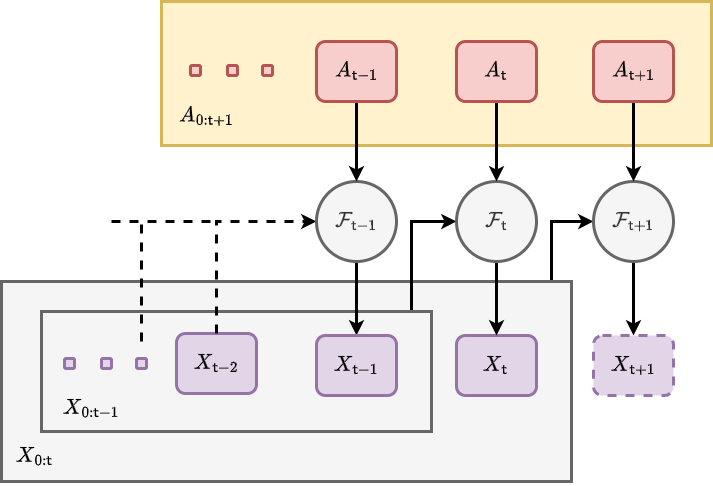
\includegraphics[width=11cm]{images/chapter-9-fundamental-loop-with-actions.drawio.png}
\caption{Graph representation of Eq.~(\ref{eq:generalised-state-actions}).}
\label{fig:fundamental-loop-with-actions}
\end{figure}

\begin{figure}[h]
\centering
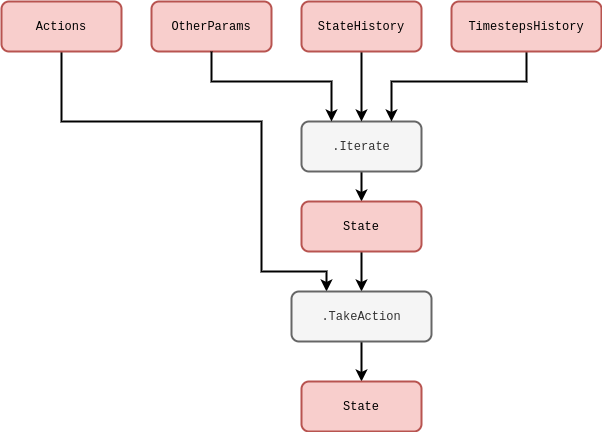
\includegraphics[width=11cm]{images/chapter-9-iterations-with-actions.drawio.png}
\caption{Code schematic of Eq.~(\ref{eq:generalised-state-actions}).}
\label{fig:iterations-with-actions}
\end{figure}

So far, Eq.~(\ref{eq:generalised-state-actions}) on its own will allow the agent to take actions that are scheduled up front through some fixed process or perhaps through user interaction via a game interface. So what's next? In order to start creating algorithms which will act on the system state for us, we need to develop a formalism which `closes the loop' by feeding information back from the stochastic process to the agent's decision-making algorithm.

If we use $A_{0:{\sf t}+1}$ a referring to the matrix of historically-taken actions which up to time ${\sf t}+1$, we can build up a more generalised, non-Markovian picture of automated interactions with the system which matches the notation we are already using for $X_{0:{\sf t}+1}$. Let us now define a Non-Markovian Decision Process (NMDP) as a probabilistic model which draws an actions matrix $A=A_{0:{\sf t}+1}$ from a `policy' distribution $\Pi_{({\sf t}+1){\sf t}}(A\vert X,\theta)$ given $X=X_{0:{\sf t}}$ and a new vector of parameters which fully specify the automated interations. Using the probabilistic notation from the previous part of the book, the joint probability that $X=X_{0:{\sf t}+1}$ and $A=A_{0:{\sf t}+1}$ at time ${\sf t}+1$ is
%%
\begin{align}
P_{{\sf t}+1}(X,A\vert z, \theta ) &= P_{{\sf t}}(X'\vert z,\theta ) \, \Pi_{({\sf t}+1){\sf t}}(A\vert X',\theta)P_{({\sf t}+1){\sf t}}(X\vert X',z,A) \label{eq:joint-prob-x-and-a} \,,
\end{align}
%%
where we recall that $P_{({\sf t}+1){\sf t}}(X\vert X',z,A)$ is the conditional probability of $X=X_{0:{\sf t}+1}$ given $X'=X_{0:{\sf t}}$ and $z$ that we have encountered before, but it now requires $A=A_{0:{\sf t}+1}$ as another given input.

By marginalising over Eq.~(\ref{eq:joint-prob-x-and-a}) we find an updated probabilistic iteration formula for the stochastic process state which now takes the influence of agent actions into account
%%
\begin{align}
P_{{\sf t}+1}(X\vert z,\theta ) &= \int_{\Omega_{{\sf t}}}{\rm d}X' \int_{\Xi_{{\sf t}+1}}{\rm d}A \, P_{{\sf t}}(X'\vert z,\theta ) \, \Pi_{({\sf t}+1){\sf t}}(A\vert X',\theta)P_{({\sf t}+1){\sf t}}(X\vert X',z,A)  \,.
\end{align}
%%

\textcolor{red}{Explain in more detail --- plus give some examples of actions before moving onto the code.}
